\documentclass{standalone}
\usepackage{tikz}
\usepackage{ctex,siunitx}
\usepackage{tkz-euclide}
\usepackage{amsmath}
\usetikzlibrary{patterns, calc}
\usetikzlibrary {decorations.pathmorphing, decorations.pathreplacing, decorations.shapes,}
\begin{document}
\small
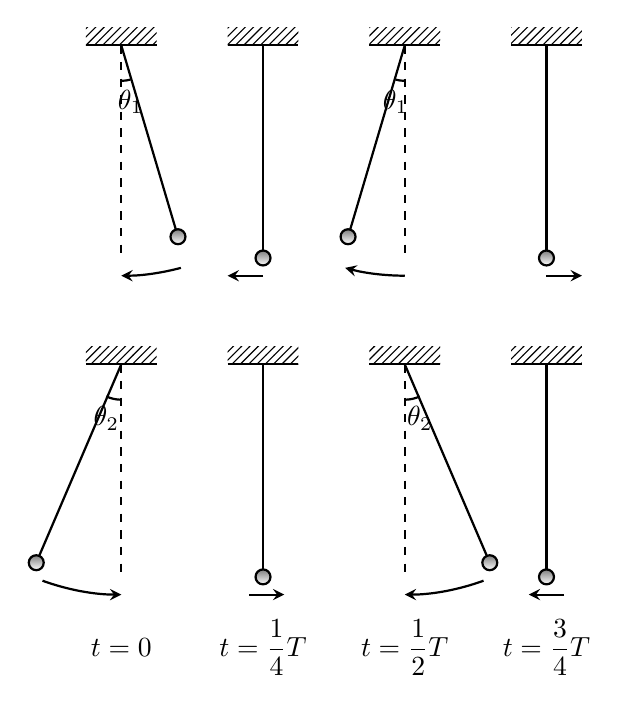
\begin{tikzpicture}[>=stealth,thick,scale=0.9]
  \fill [pattern = north east lines] (-4,0) rectangle (-3,.25);
  \fill [pattern = north east lines] (-2,0) rectangle (-1,.25);
  \fill [pattern = north east lines] (0,0) rectangle (1,.25);
  \fill [pattern = north east lines] (2,0) rectangle (3,.25);
  \draw(-4,0)--(-3,0);  \draw(-2,0)--(-1,0); \draw(0,0)--(1,0); \draw(2,0)--(3,0); 
  \draw[dashed](-3.5,0)--(-3.5,-3);  \draw(-1.5,0)--(-1.5,-3);  
  \draw[dashed](.5,0)--(.5,-3);       \draw(2.5,0)--(2.5,-3);
  \draw(-3.5,0)--(-3+.3,-2.7);  \draw(.5,0)--(0-.3,-2.7);
  \draw[shade] (-1.5,-3) circle  (3pt);
  \draw[shade] (2.5,-3) circle  (3pt);
  \draw[shade] (-3+.3,-2.7) circle  (3pt);
  \draw[shade] (0-.3,-2.7) circle  (3pt);
  \draw (-3.5,-.5) arc (270:285:.5) node [below]{$\theta_1$};
  \draw (.5,-.5) arc (270:255:.5) node [below]{$\theta_1$};
  \draw [<-](-3.5,-3.25) arc (270:285:3.25);
  \draw [->](.5,-3.25) arc (270:255:3.25);
  \draw [->](-1.5,-3.25)--(-2,-3.25);
  \draw [<-](3,-3.25)--(2.5,-3.25);
  \node at (-4,-4){~~};
  \begin{scope}[yshift=-4.5cm]
    \fill [pattern = north east lines] (-4,0) rectangle (-3,.25);
    \fill [pattern = north east lines] (-2,0) rectangle (-1,.25);
    \fill [pattern = north east lines] (0,0) rectangle (1,.25);
    \fill [pattern = north east lines] (2,0) rectangle (3,.25);
    \draw(-4,0)--(-3,0);  \draw(-2,0)--(-1,0); \draw(0,0)--(1,0); \draw(2,0)--(3,0); 
    \draw[dashed](-3.5,0)--(-3.5,-3);  \draw(-1.5,0)--(-1.5,-3);  
    \draw[dashed](.5,0)--(.5,-3);       \draw(2.5,0)--(2.5,-3);
    \draw(-3.5,0)--(-3.5-1.2,-2.8);  \draw(.5,0)--(.5+1.2,-2.8);
    \draw[shade] (-1.5,-3) circle  (3pt);
    \draw[shade] (2.5,-3) circle  (3pt);
    \draw[shade] (-3.5-1.2,-2.8) circle  (3pt);
    \draw[shade] (.5+1.2,-2.8) circle  (3pt);
    \draw (-3.5,-.5) arc (270:245:.5) node [below]{$\theta_2$};
    \draw (.5,-.5) arc (270:295:.5) node [below]{$\theta_2$};
    \draw [<-](-3.5,-3.25) arc (270:250:3.25);
    \draw [<-](.5,-3.25) arc (270:290:3.25);
    \draw [<-](-1.2,-3.25)--(-1.7,-3.25);
    \draw [->](2.75,-3.25)--(2.25,-3.25);
    \node at (-3.5,-4){$t=0$};\node at (-1.5,-4){$t=\dfrac{1}{4}T$};
    \node at (.5,-4){$t=\dfrac{1}{2}T$};\node at (2.5,-4){$t=\dfrac{3}{4}T$};
  \end{scope}
\end{tikzpicture}
\end{document}